%\section{VC++ 6.0 IDE}
%\label{sec:vc}
%\begin{frame}<beamer>
%    \frametitle{Outline}
%    \tableofcontents[currentsection]
%\end{frame}
%
%
%\begin{frame}{VC++ 6.0 IDE (1)}
%	\begin{figure}
%		\begin{center}
%			\begin{figure}
%				\includegraphics[width=0.8\linewidth]{figs/vc1.pdf}
%			\end{figure}
%		\end{center}
%	\end{figure}
%	\begin{itemize}
%		\item {Create/New a C project}
%	\end{itemize}
%\end{frame}
%
%\begin{frame}{VC++ 6.0 IDE (2)}
%	\begin{figure}
%		\begin{center}
%			\begin{figure}
%				\includegraphics[width=0.8\linewidth]{figs/vc2.pdf}
%			\end{figure}
%		\end{center}
%	\end{figure}
%	\begin{itemize}
%		\item {Choose to create "\textcolor{red}{Win32 Console Application}"}
%		\item {Give a meaningful name for your project, such as "test1"}
%	\end{itemize}
%\end{frame}
%
%\begin{frame}{VC++ 6.0 IDE (3)}
%	\begin{figure}
%		\begin{center}
%			\begin{figure}
%				\includegraphics[width=0.8\linewidth]{figs/vc3.pdf}
%			\end{figure}
%		\end{center}
%	\end{figure}
%	\begin{itemize}
%		\item {Choose to create "\textcolor{red}{an empty project}"}
%	\end{itemize}
%\end{frame}
%
%\begin{frame}{VC++ 6.0 IDE (4)}
%	\begin{figure}
%		\begin{center}
%			\begin{figure}
%				\includegraphics[width=0.8\linewidth]{figs/vc4.pdf}
%			\end{figure}
%		\end{center}
%	\end{figure}
%	\begin{itemize}
%		\item {Create C files under the your current project}
%		\item {Give a meaningful and unique name for your file}
%	\end{itemize}
%\end{frame}
%
%\begin{frame}{VC++ 6.0 IDE (5)}
%	\begin{figure}
%		\begin{center}
%			\begin{figure}
%				\includegraphics[width=0.8\linewidth]{figs/vc5.pdf}
%			\end{figure}
%		\end{center}
%	\end{figure}
%	\begin{itemize}
%		\item {Edit your current C file}
%		\item {Keywords are in \textcolor{blue}{blue}}
%	\end{itemize}
%\end{frame}
%
%\begin{frame}{VC++ 6.0 IDE (6)}
%	\begin{figure}
%		\begin{center}
%			\begin{figure}
%				\includegraphics[width=0.8\linewidth]{figs/vc6.pdf}
%			\end{figure}
%		\end{center}
%	\end{figure}
%	\begin{itemize}
%		\item {When there is something wrong during compiling}
%		\item {It will be shown in the window below}
%	\end{itemize}
%\end{frame}
%
%\begin{frame}{VC++ 6.0 IDE (7)}
%	\begin{figure}
%		\begin{center}
%			\begin{figure}
%				\includegraphics[width=0.8\linewidth]{figs/flow.pdf}
%			\end{figure}
%		\end{center}
%	\end{figure}
%\end{frame}
%
%\begin{frame}
%\frametitle{Hello world (1)}
%\begin{itemize}
%	\item {Try following code:}
%	\begin{enumerate}
%		\item {\#include $<$stdio.h$>$}
%		\item {int~main(~)}
%		\item {\{}
%		\item {~~~printf("Hello world$\setminus$n");}
%		\item {\}}
%	\end{enumerate}
%\end{itemize}
%\end{frame}
%
%\begin{frame}
%\frametitle{Hello world (2)}
%\begin{itemize}
%	\item {Try following code:}
%	\begin{enumerate}
%		\item {\#include $<$stdio.h$>$}
%		\item {int~main(~)}
%		\item {\{}
%		\item {~~~printf("Hello China$\setminus$n");}
%		\item {~~~printf("Hello world$\setminus$n");}
%		\item {~~~printf("Hello universe$\setminus$n");}
%		\item {\}}
%	\end{enumerate}
%\end{itemize}
%\begin{itemize}
%	\item {This is an experiment}
%	\item {Based on this great experiment, we know that}
%	\item {\textcolor{red}{Codes are executed from top to bottom}}
%\end{itemize}
%\end{frame}

\section{Codeblocks IDE}
\label{sec:cb}
\begin{frame}<beamer>
    \frametitle{Outline}
    \tableofcontents[currentsection]
\end{frame}

\begin{frame}{Codeblocks}
\begin{itemize}
	\item {It is free software, available at following link}
\end{itemize}
\begin{center}
\href{http://121.192.176.204/sourceforge.net/projects/codeblocks/files/Binaries/16.01/Windows/codeblocks-16.01mingw-setup.exe}{\textcolor{blue}{\underline{CodeBlocks 16.01 Windows binary}}}
\end{center}
\begin{itemize}
	\item {Lightweiht and stable}
	\item {Cross platform: Linux, Windows and MacOS}
\end{itemize}
\end{frame}

\begin{frame}{Compiler Setup}
	\begin{figure}
		\begin{center}
			\begin{figure}
				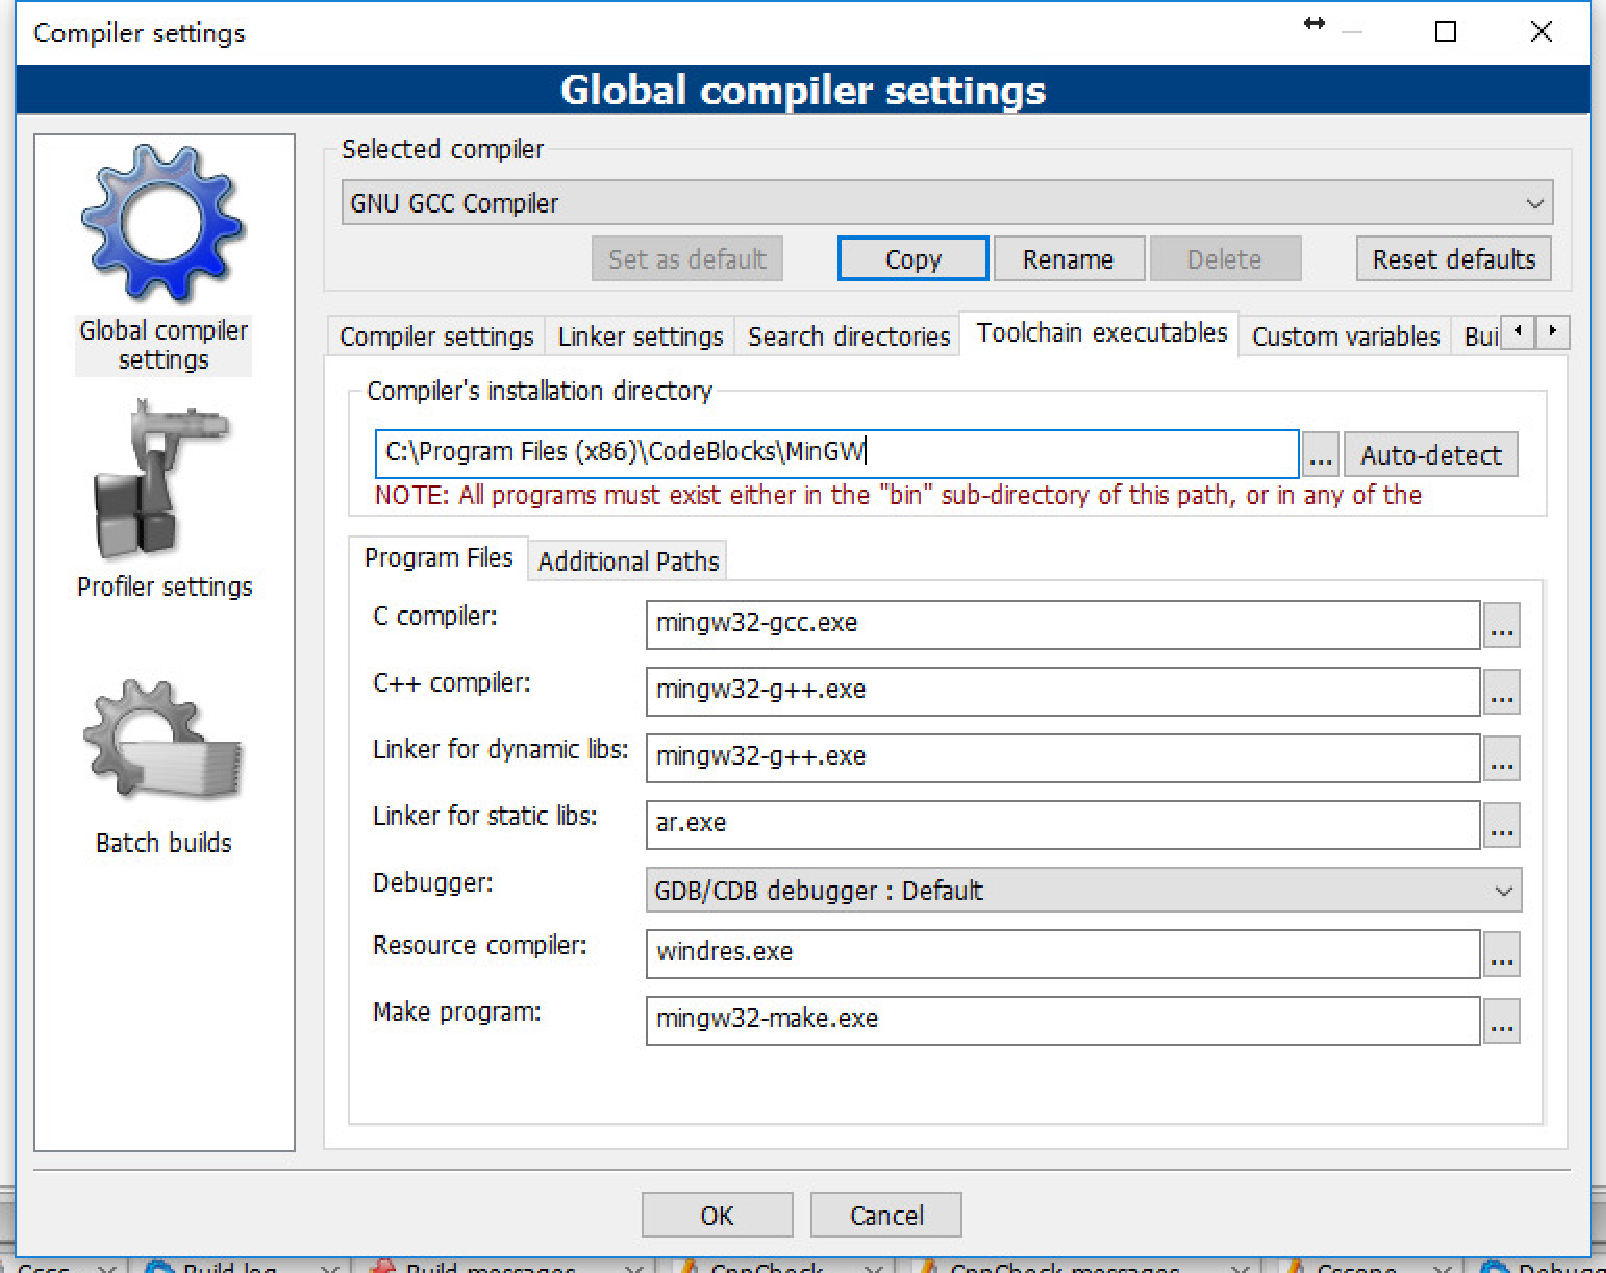
\includegraphics[width=0.6\linewidth]{figs/cbx0.pdf}
			\end{figure}
		\end{center}
	\end{figure}
	\begin{enumerate}
		\item {Go to menu: Settings$\rightarrow$Compiler Settings$\rightarrow$\textcolor{red}{Toolchain Executables}}
		\item {Type in the path for mingw compiler, e.g., C:/Program Files (x86)/CodeBlocks/MingW/}
	\end{enumerate}
	
\end{frame}


\begin{frame}{Create a project: step 1}
	\begin{figure}
		\begin{center}
			\begin{figure}
				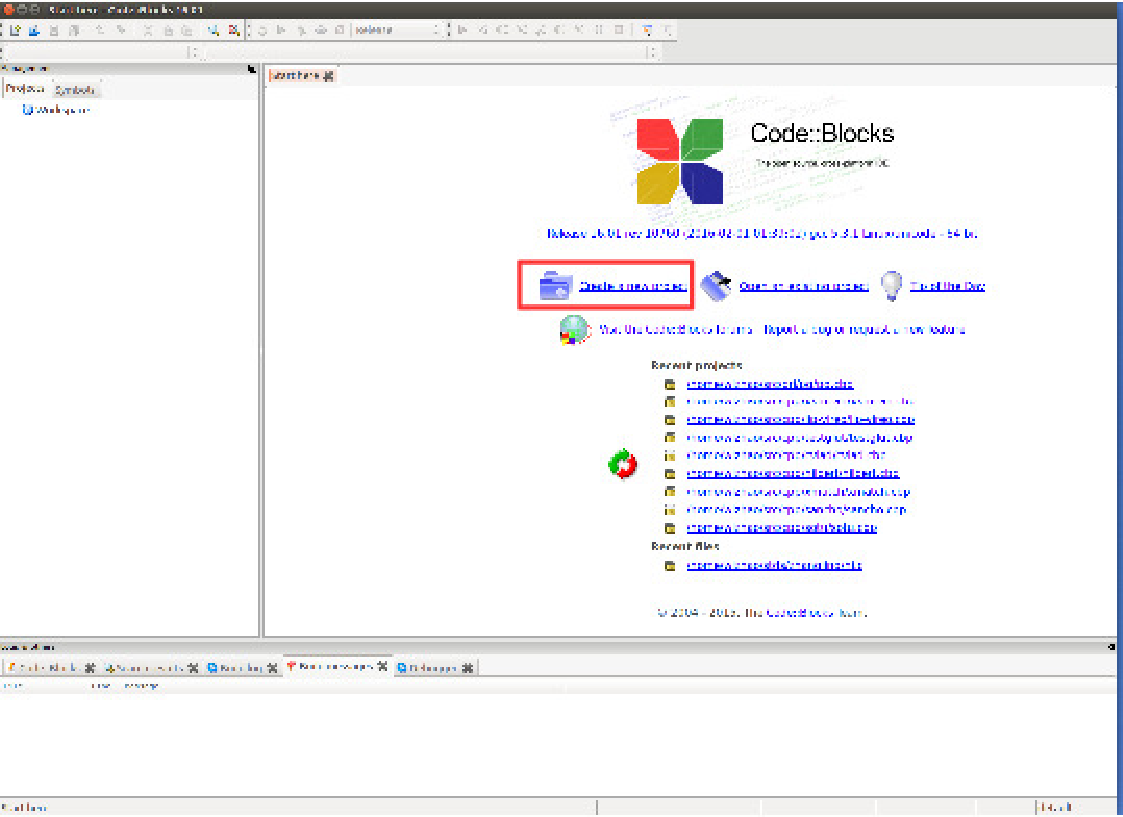
\includegraphics[width=0.8\linewidth]{figs/cbx1.pdf}
			\end{figure}
		\end{center}
	\end{figure}
	\begin{itemize}
		\item {Create/New a C project}
	\end{itemize}
\end{frame}

\begin{frame}{Create a project: step 2}
	\begin{figure}
		\begin{center}
			\begin{figure}
				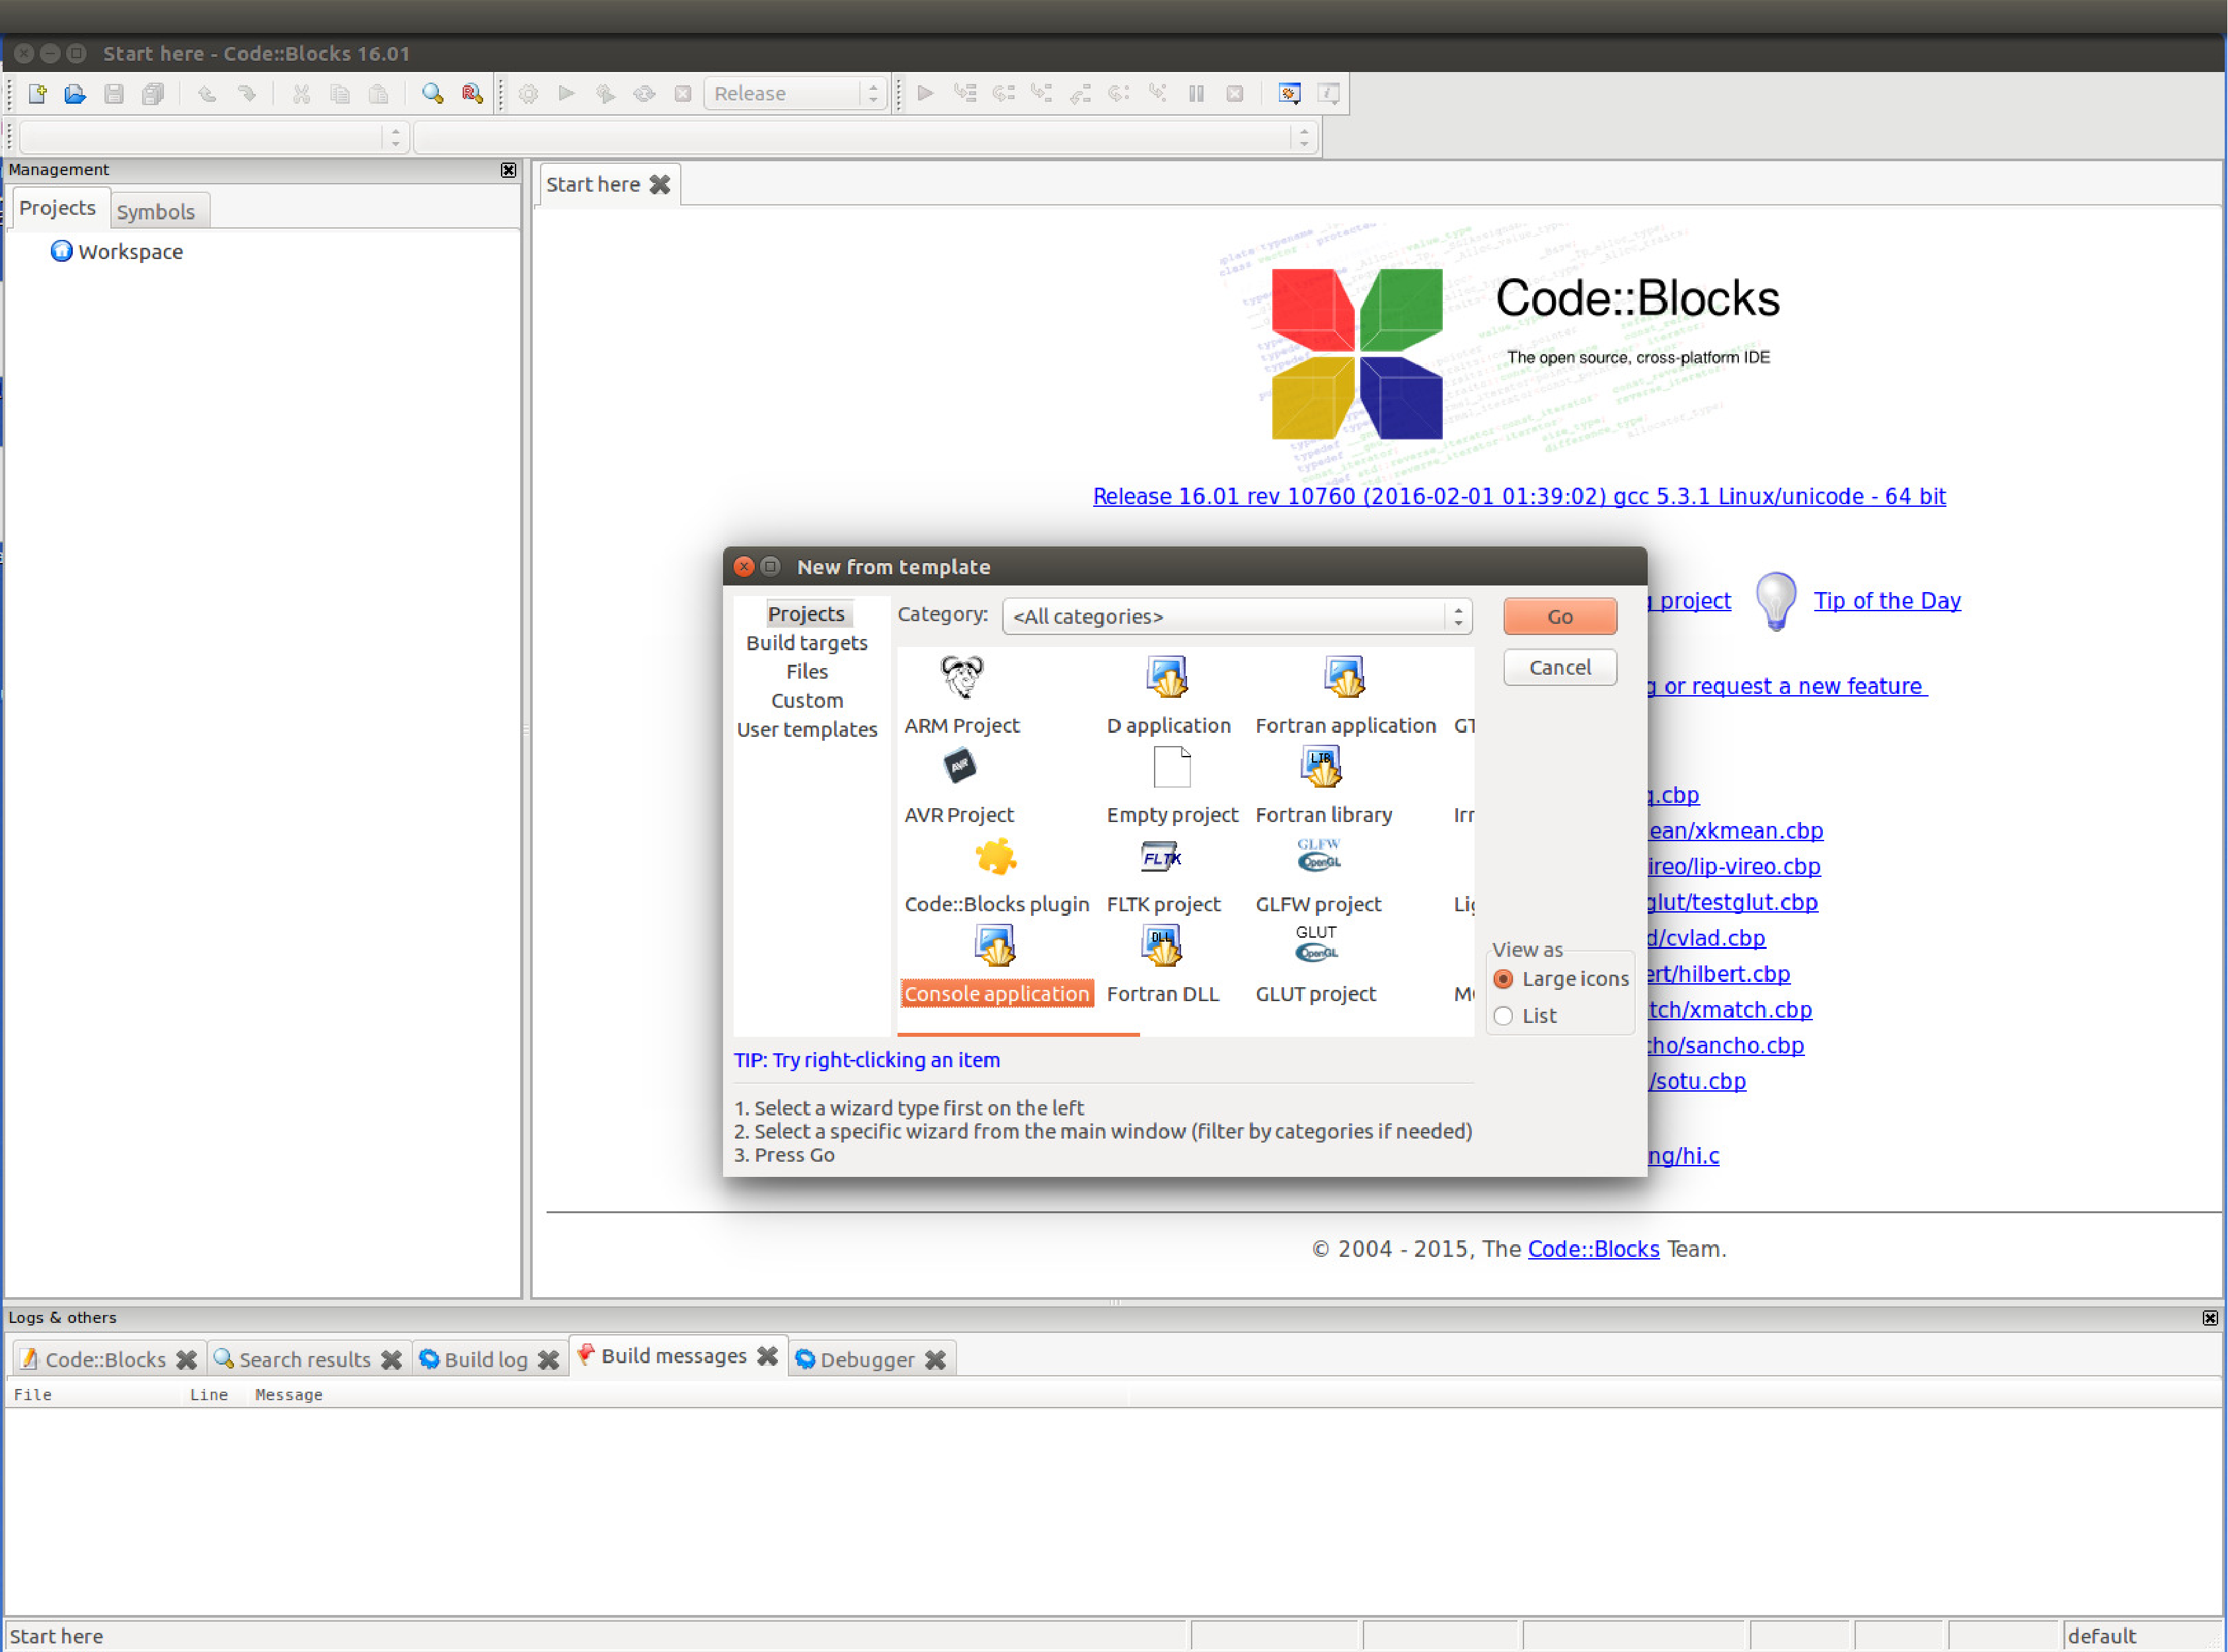
\includegraphics[width=0.8\linewidth]{figs/cb2.pdf}
			\end{figure}
		\end{center}
	\end{figure}
	\begin{itemize}
		\item {Choose project type ``Console application''}
	\end{itemize}
\end{frame}

\begin{frame}{Create a project: step 3}
	\begin{figure}
		\begin{center}
			\begin{figure}
				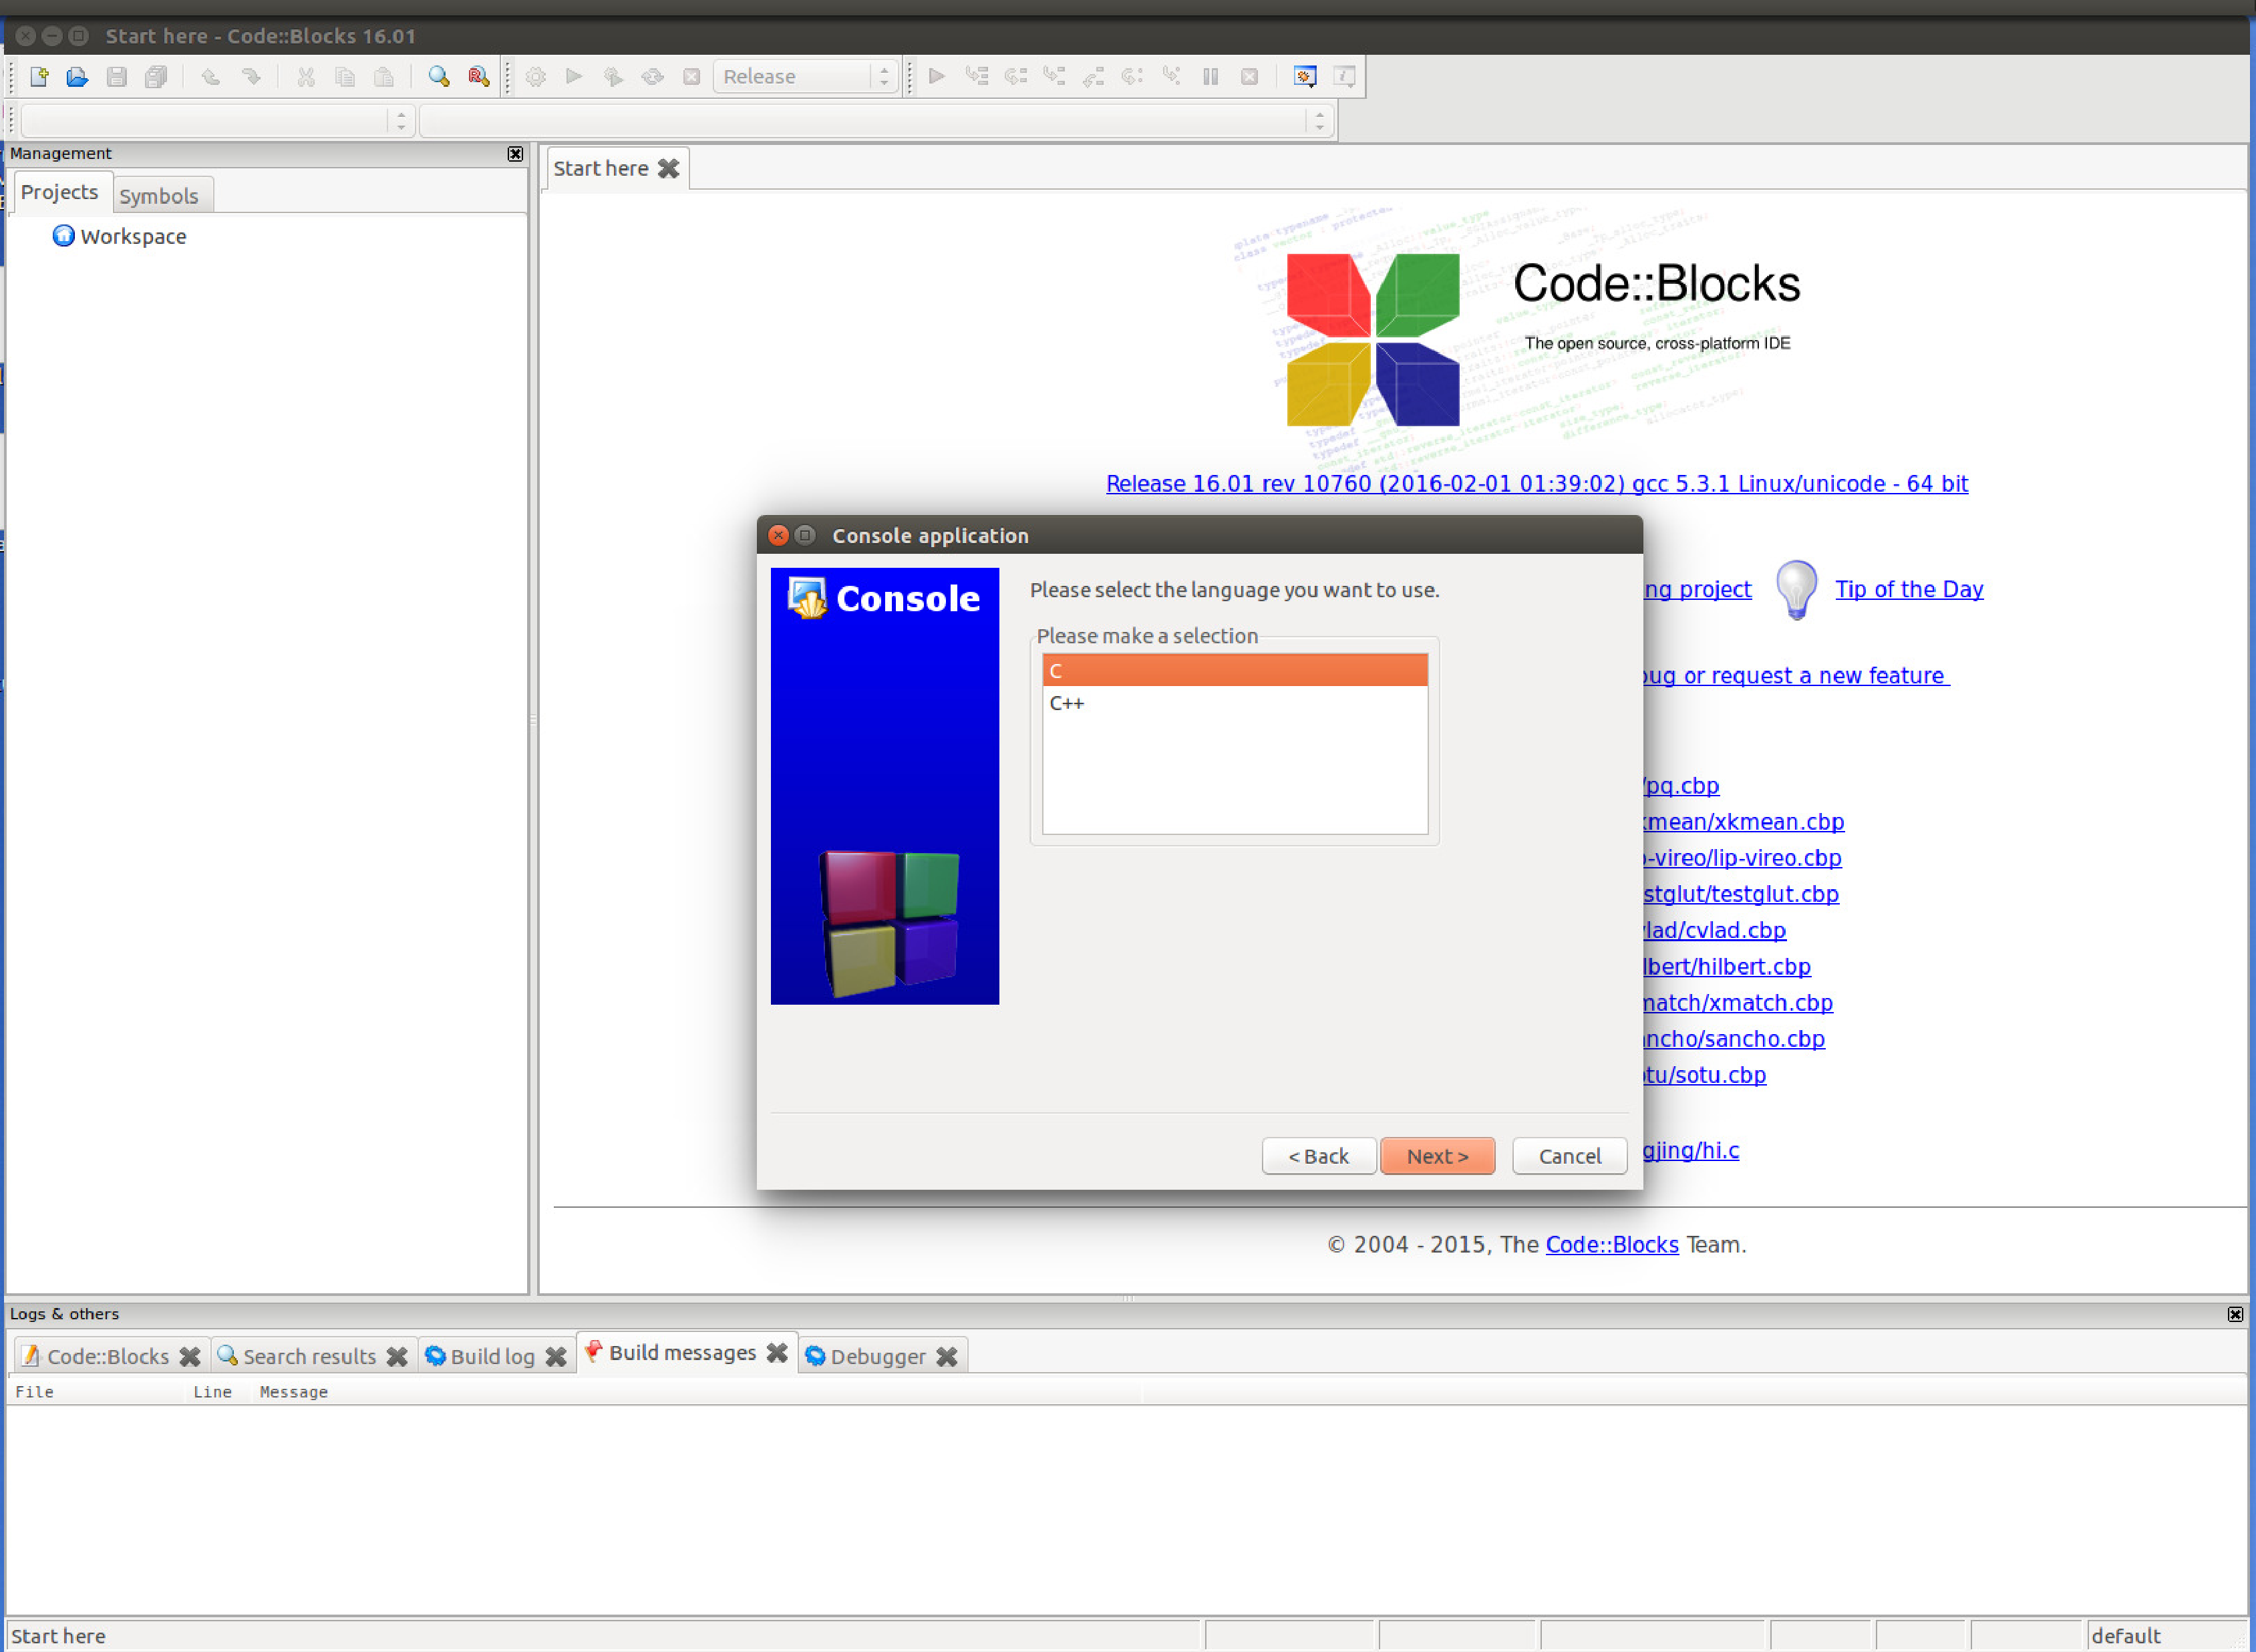
\includegraphics[width=0.8\linewidth]{figs/cb3.pdf}
			\end{figure}
		\end{center}
	\end{figure}
	\begin{itemize}
		\item {Set it as a ``C'' project}
	\end{itemize}
\end{frame}

\begin{frame}{Create a project: step 4}
	\begin{figure}
		\begin{center}
			\begin{figure}
				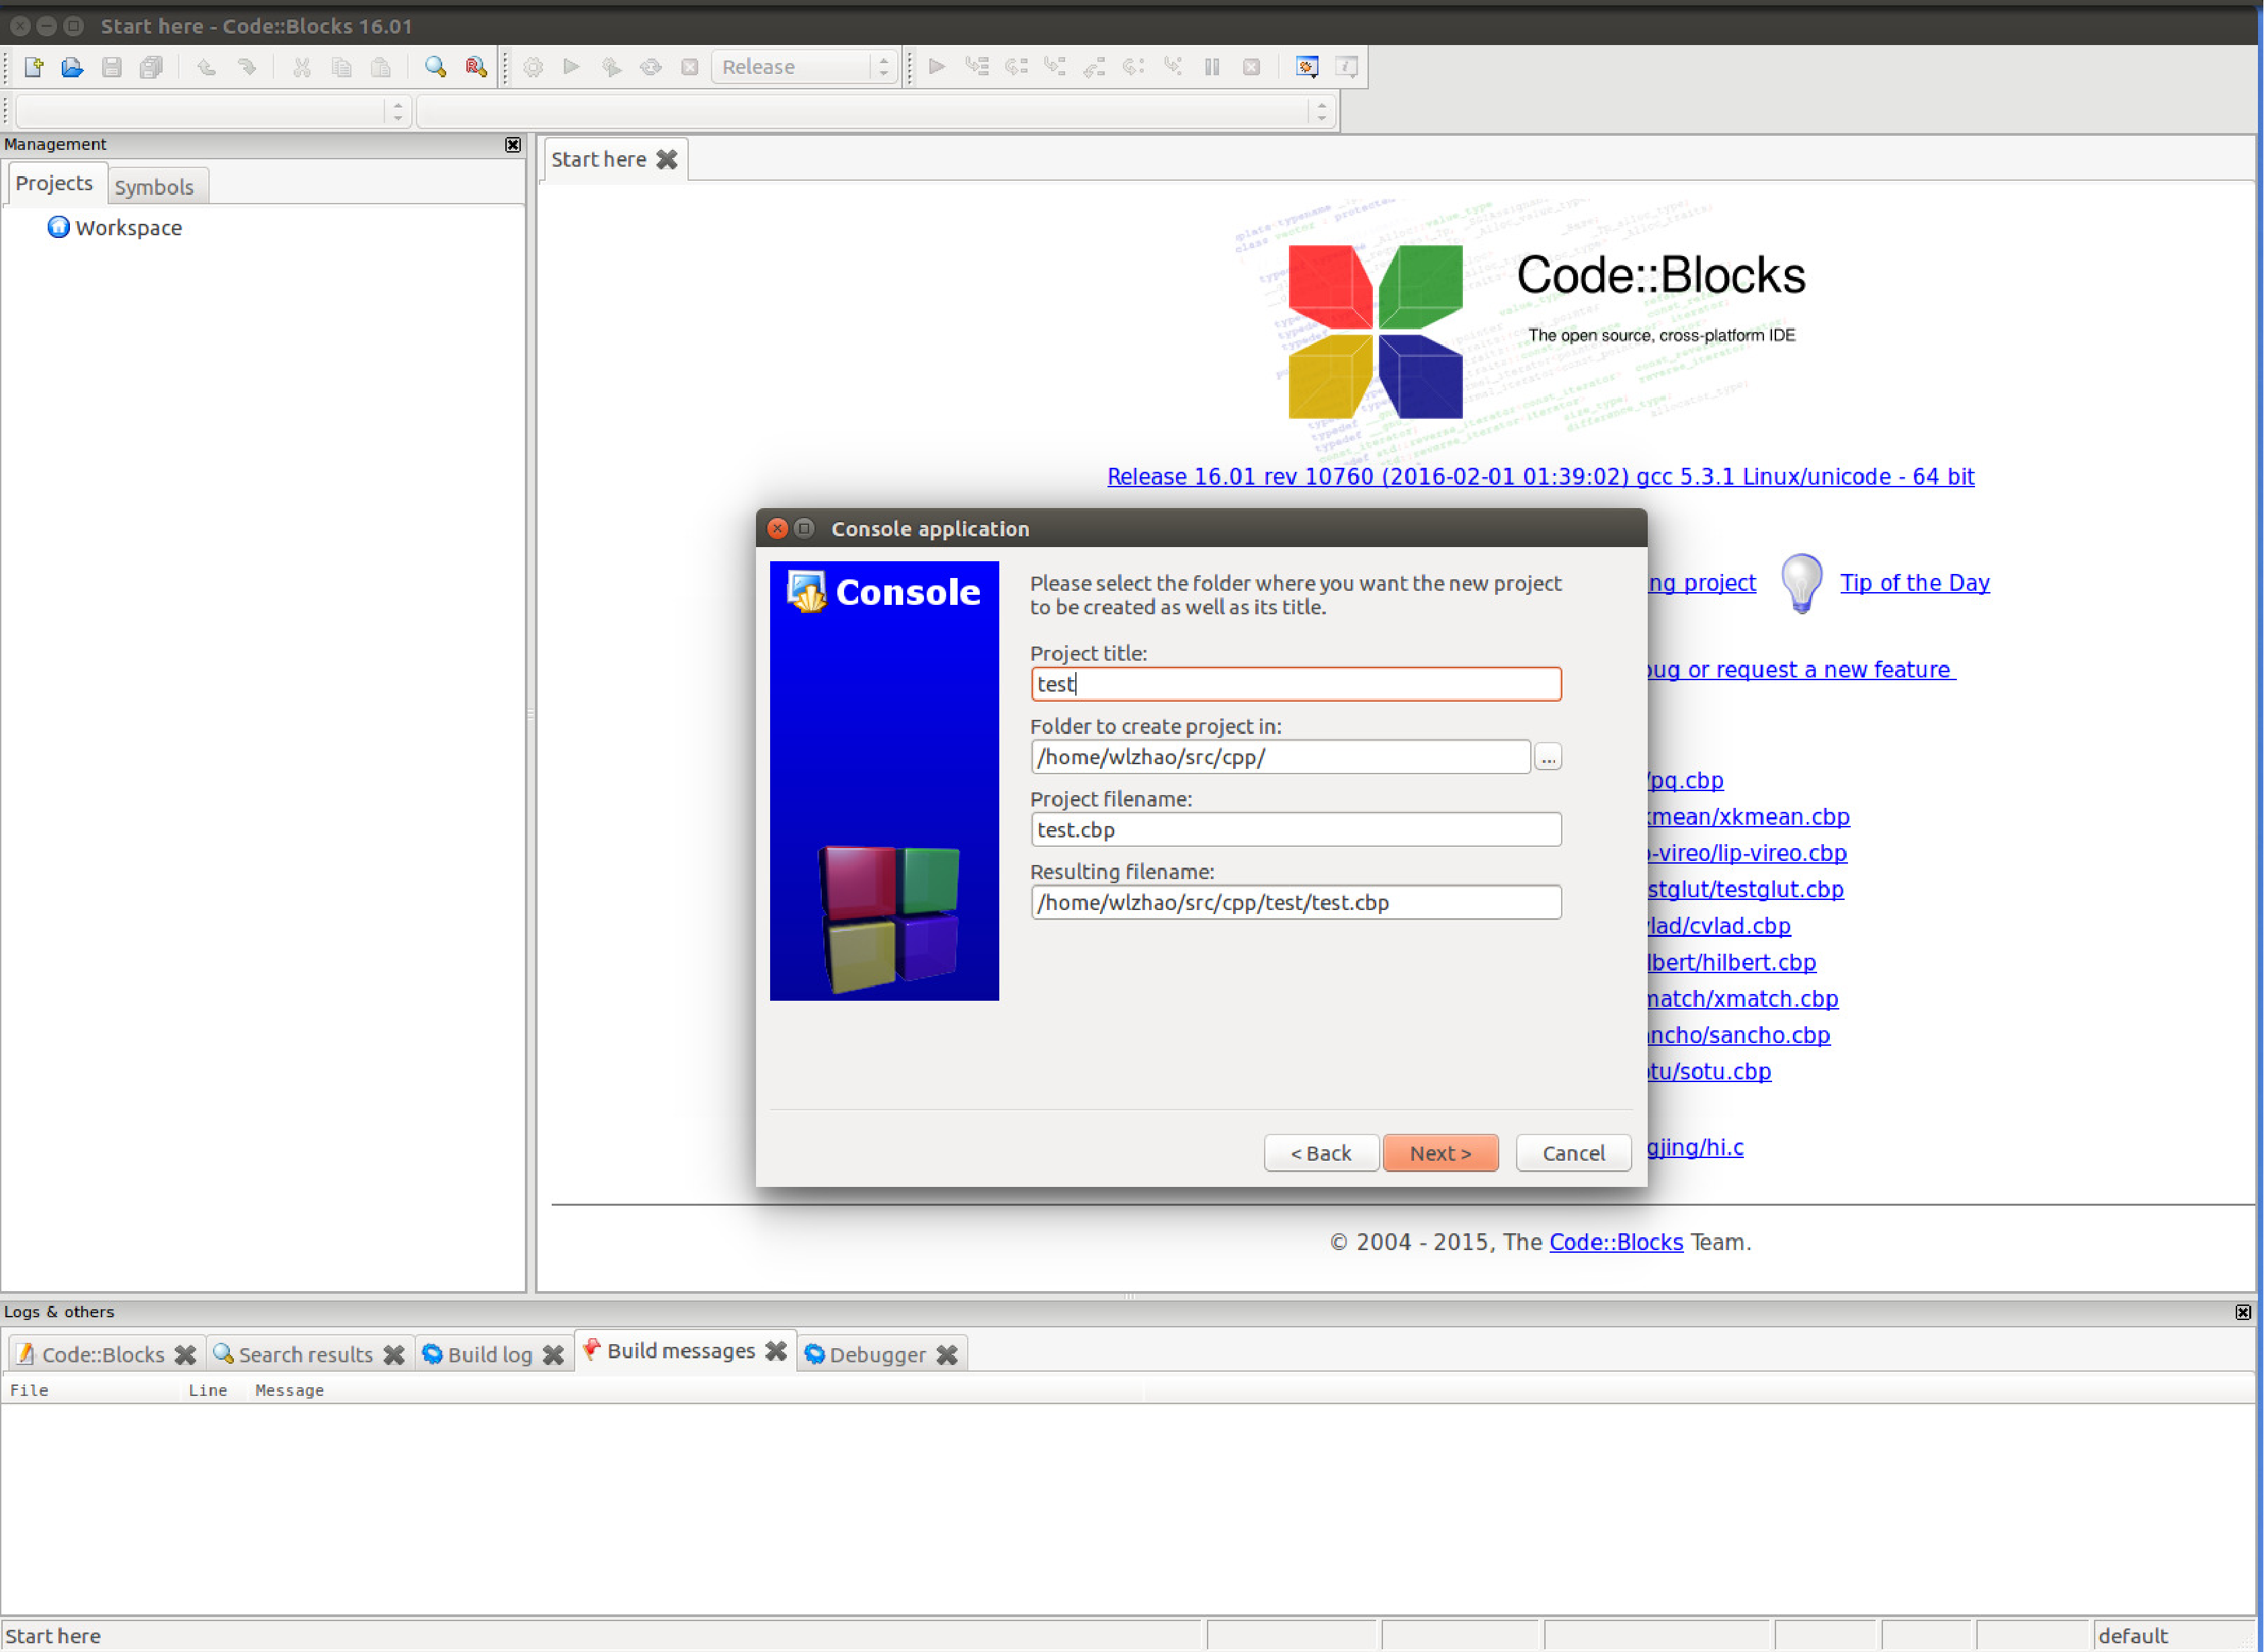
\includegraphics[width=0.8\linewidth]{figs/cb4.pdf}
			\end{figure}
		\end{center}
	\end{figure}
	\begin{itemize}
		\item {Give a name for your project}
	\end{itemize}
\end{frame}

\begin{frame}{Create a project: step 5}
	\begin{figure}
		\begin{center}
			\begin{figure}
				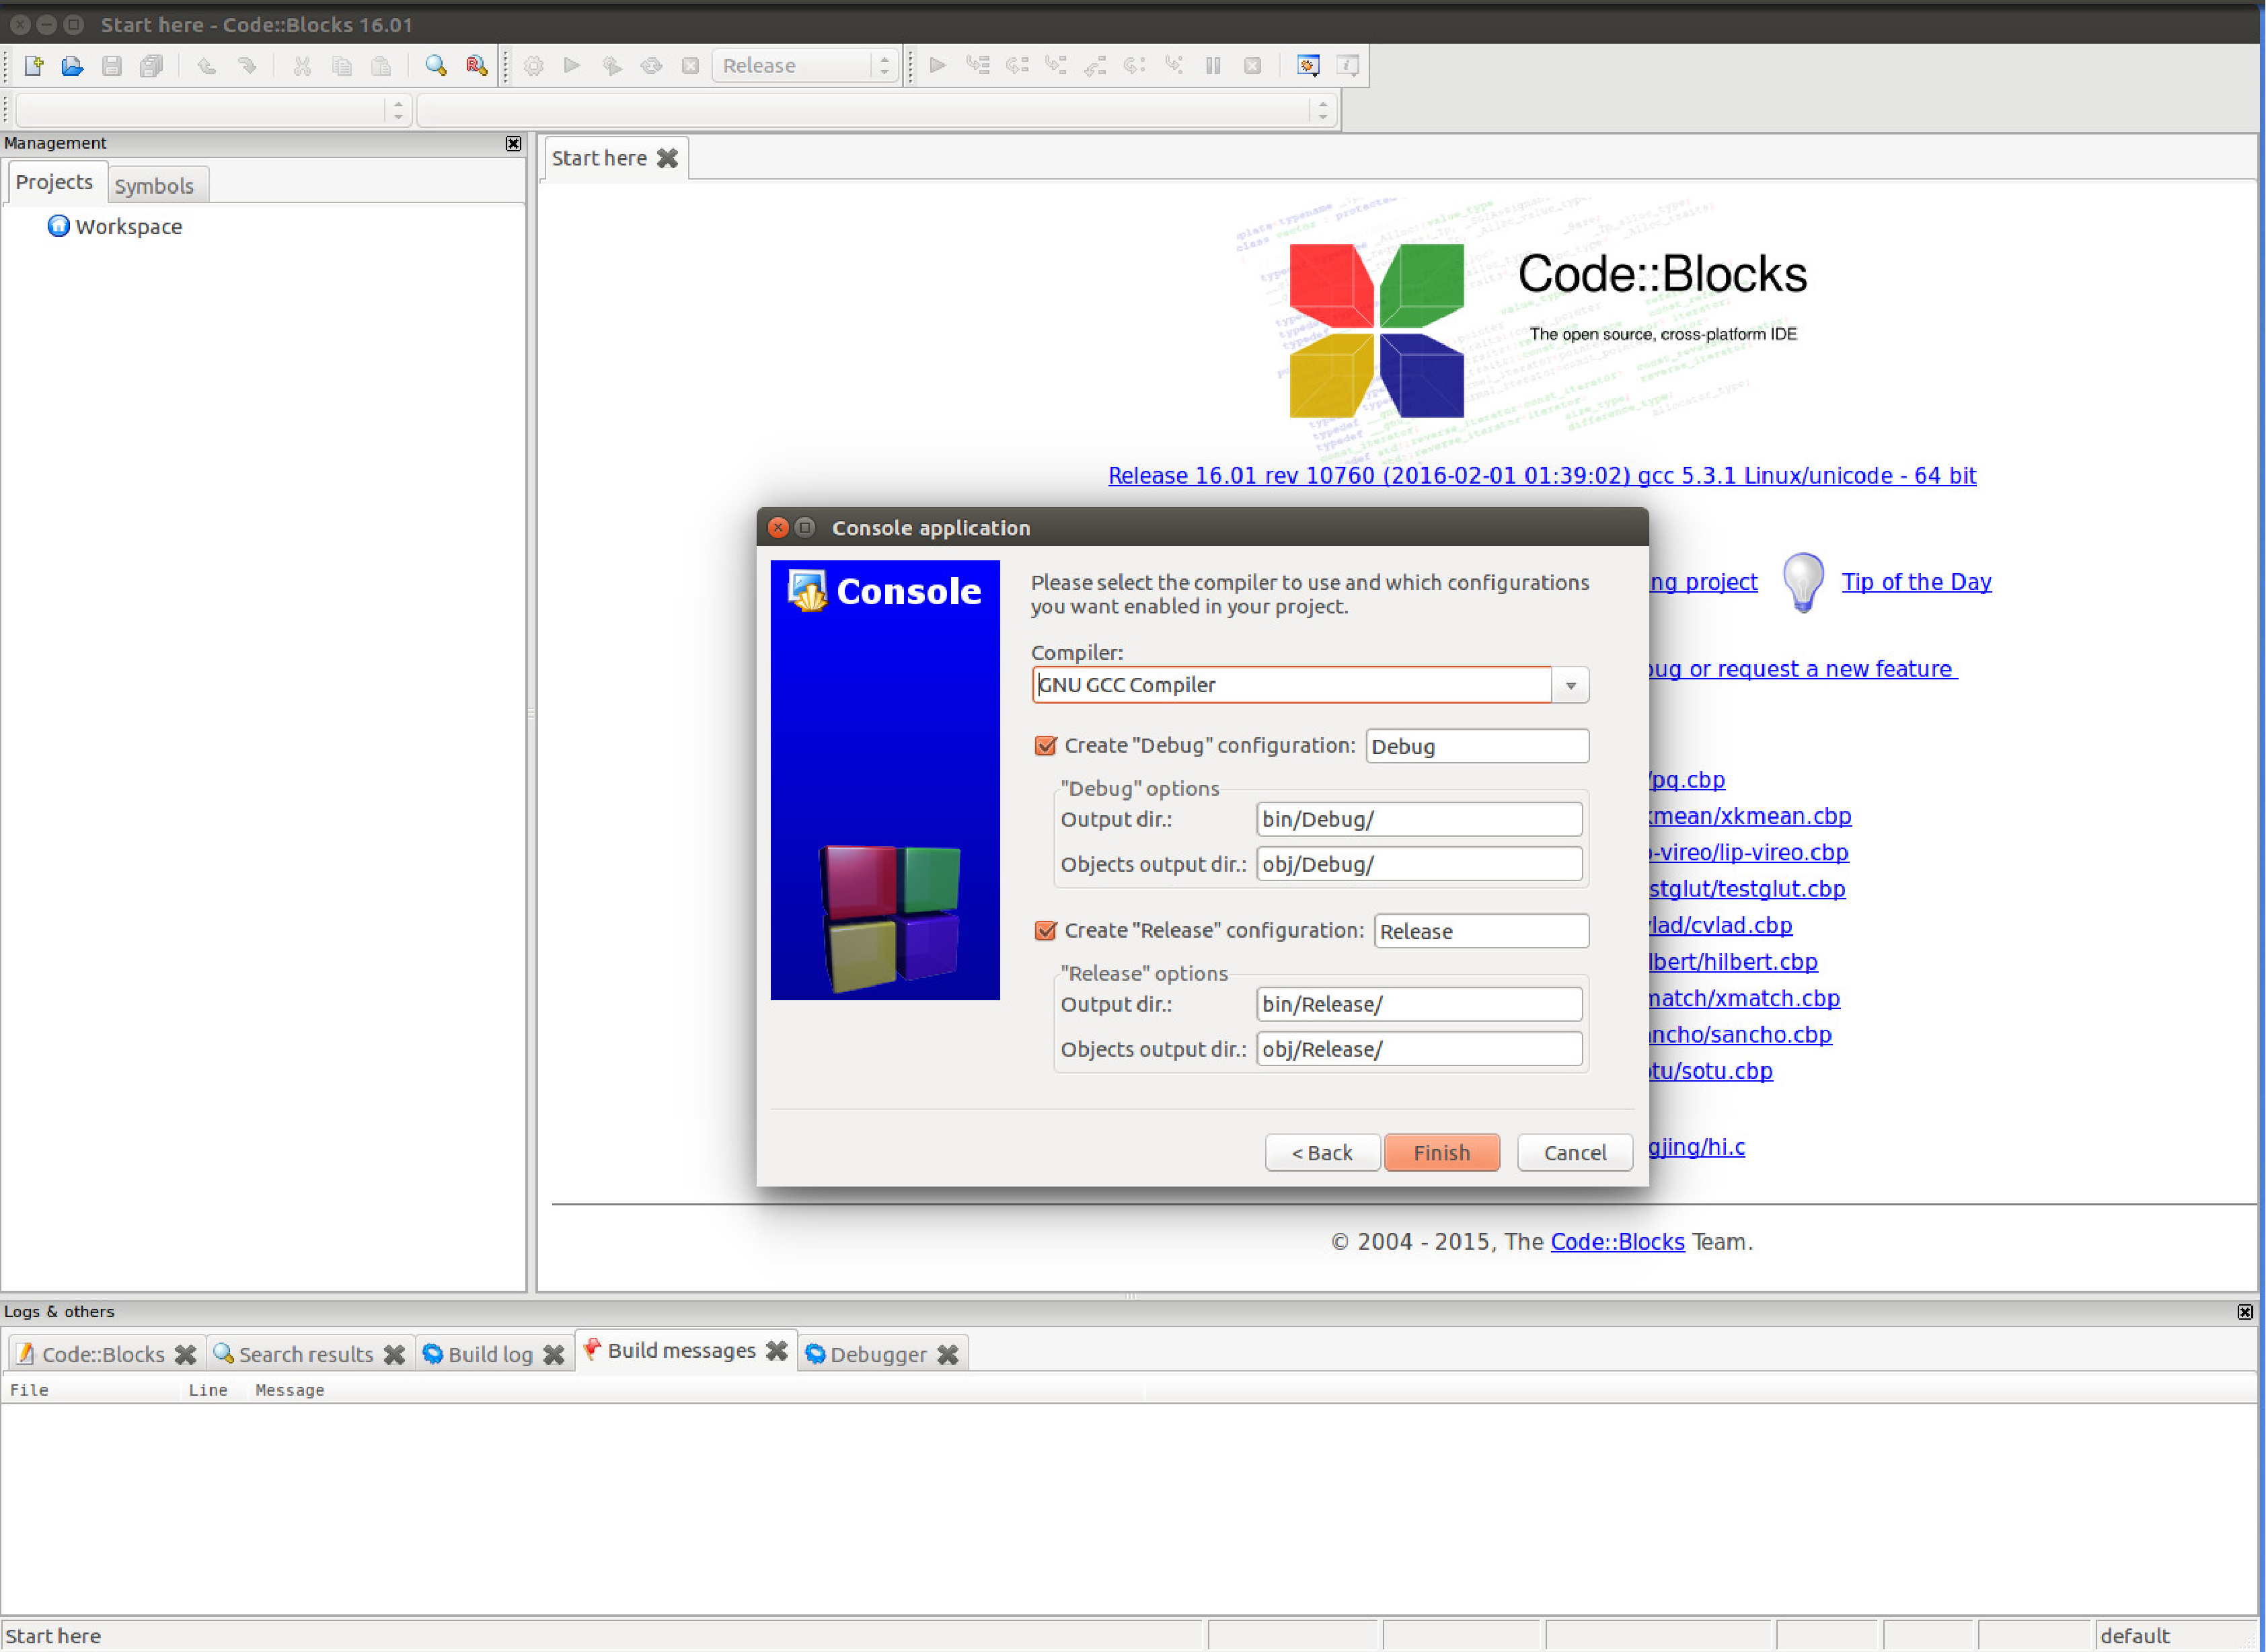
\includegraphics[width=0.8\linewidth]{figs/cb5.pdf}
			\end{figure}
		\end{center}
	\end{figure}
	\begin{itemize}
		\item {Choose ``C'' compiler for your project}
	\end{itemize}
\end{frame}

\begin{frame}{Create a project: step 6}
	\begin{figure}
		\begin{center}
			\begin{figure}
				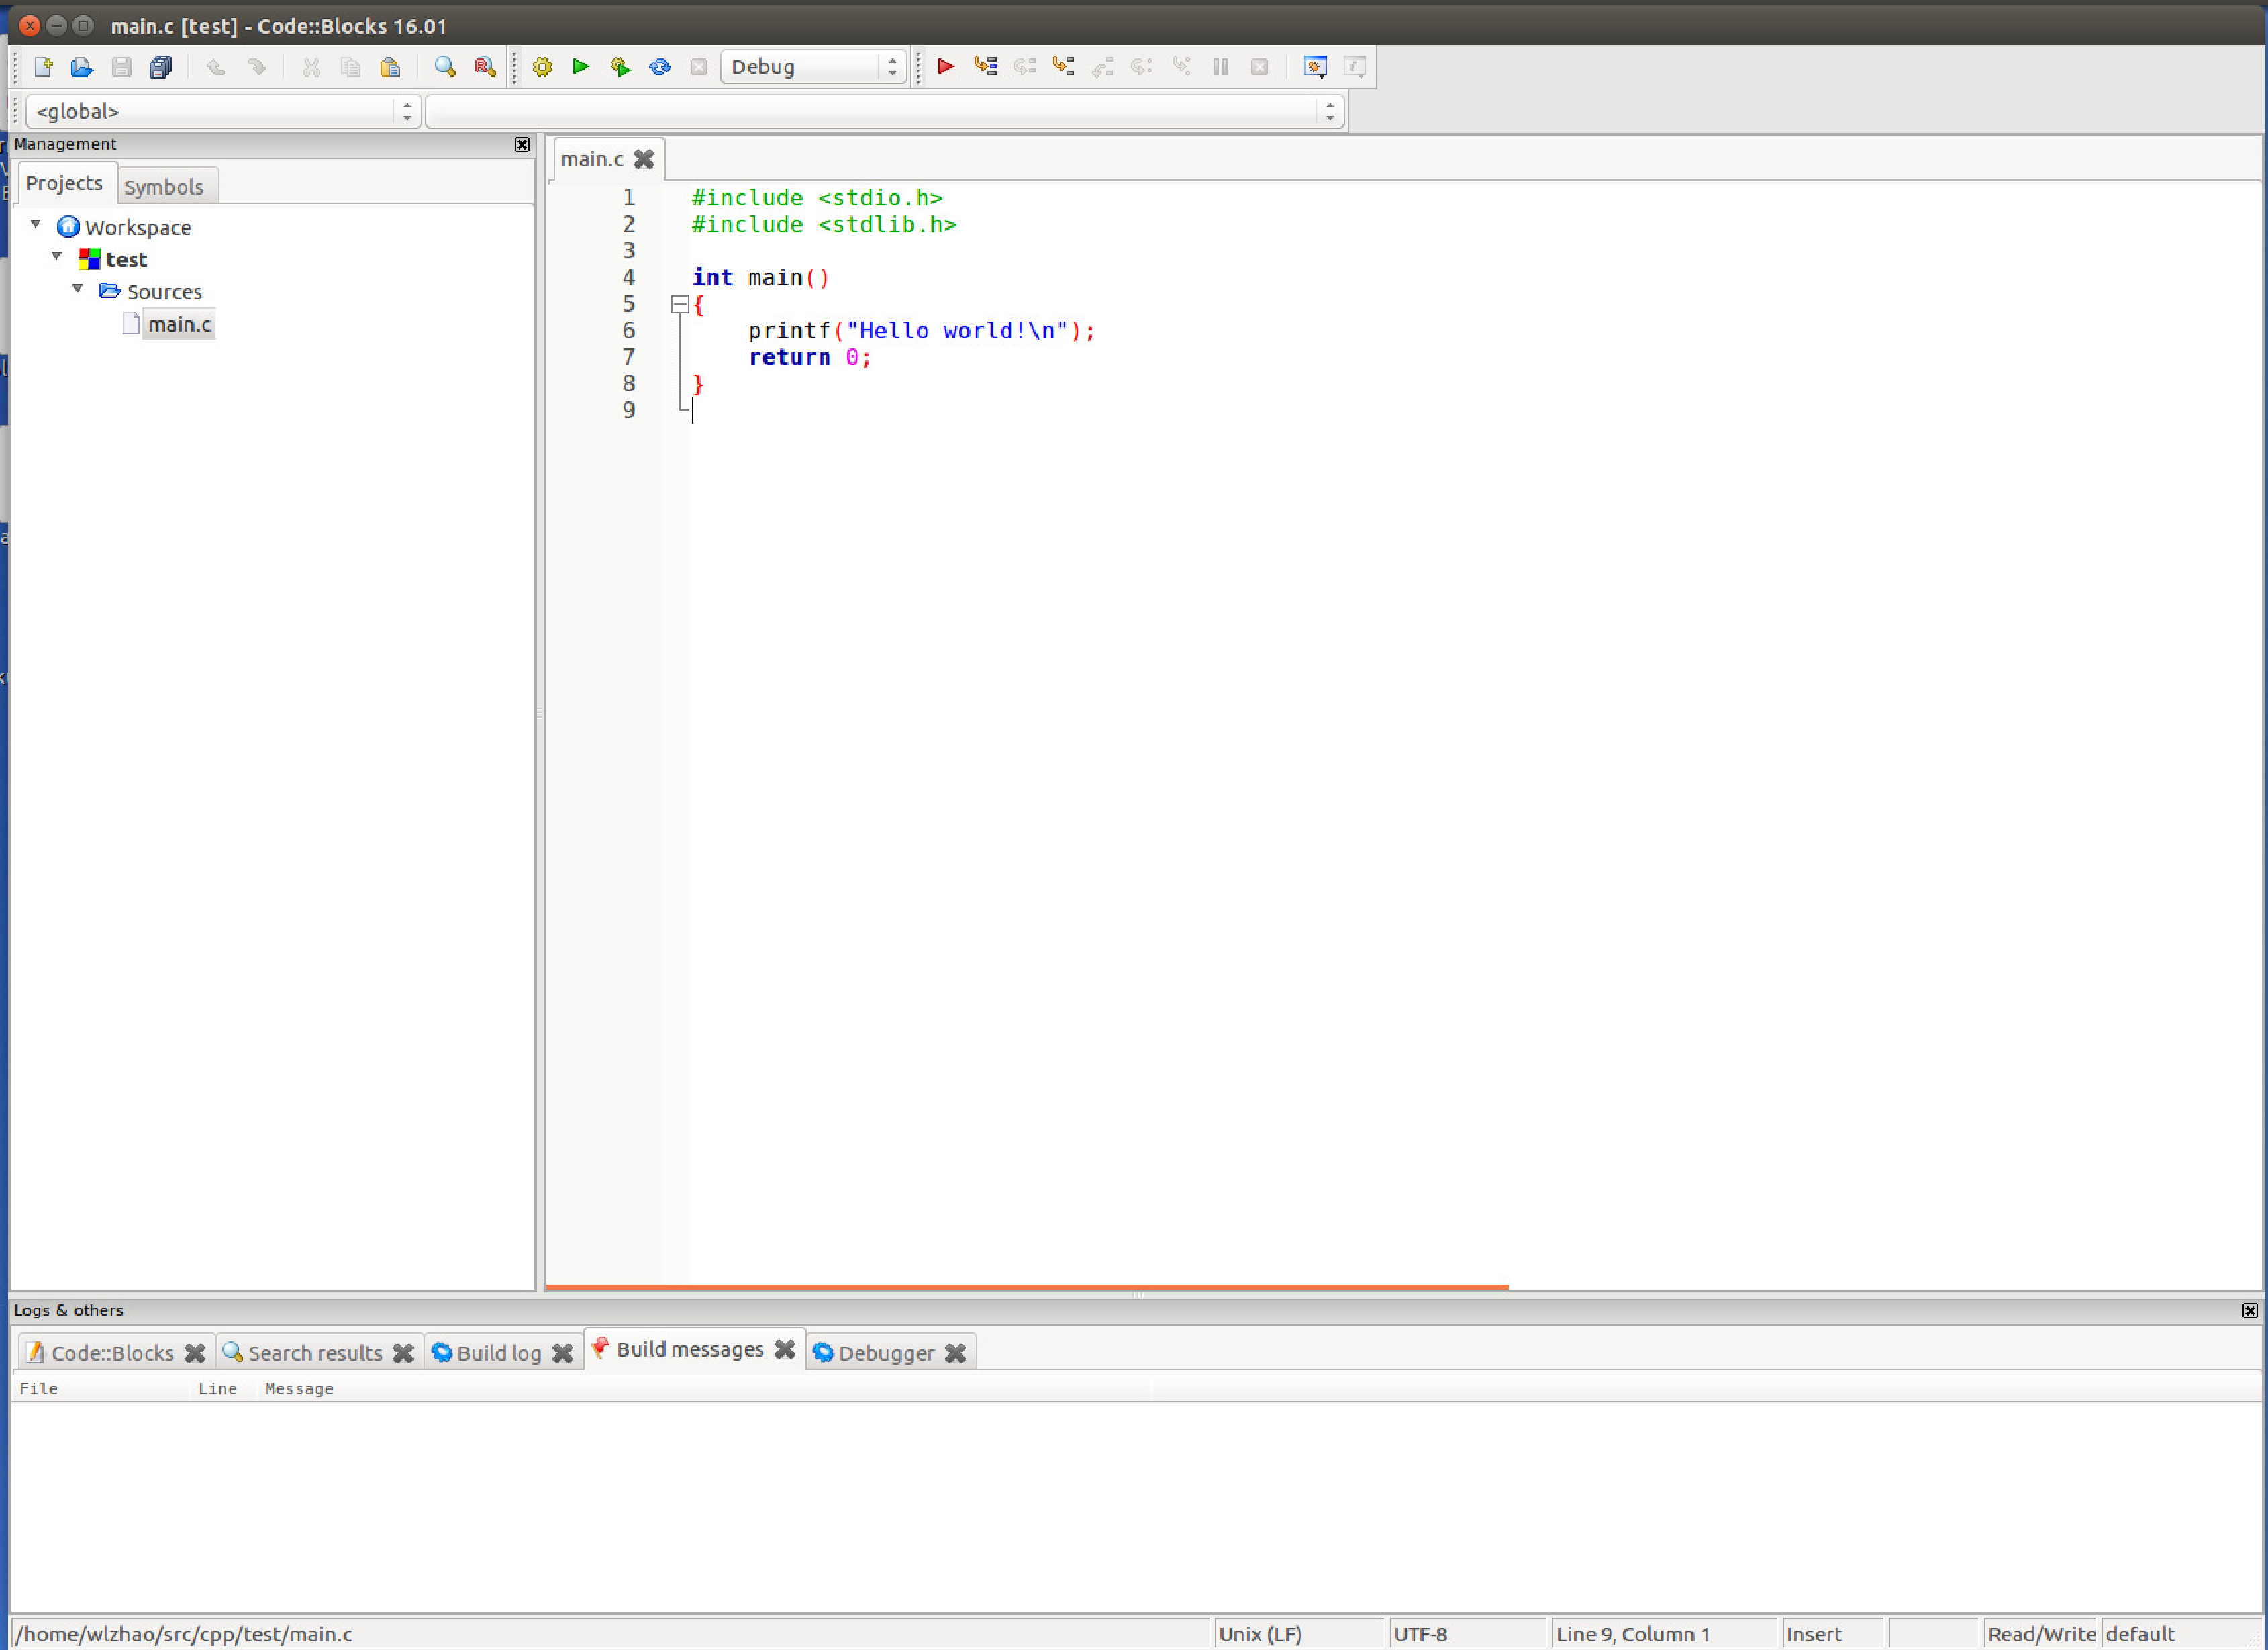
\includegraphics[width=0.8\linewidth]{figs/cb6.pdf}
			\end{figure}
		\end{center}
	\end{figure}
	\begin{itemize}
		\item {Start to work with your project}
	\end{itemize}
\end{frame}

\section{Visual Studio Code}
\label{sec:vs}
\begin{frame}{Main interface of VS code}
	\begin{figure}
		\begin{center}
			\begin{figure}
				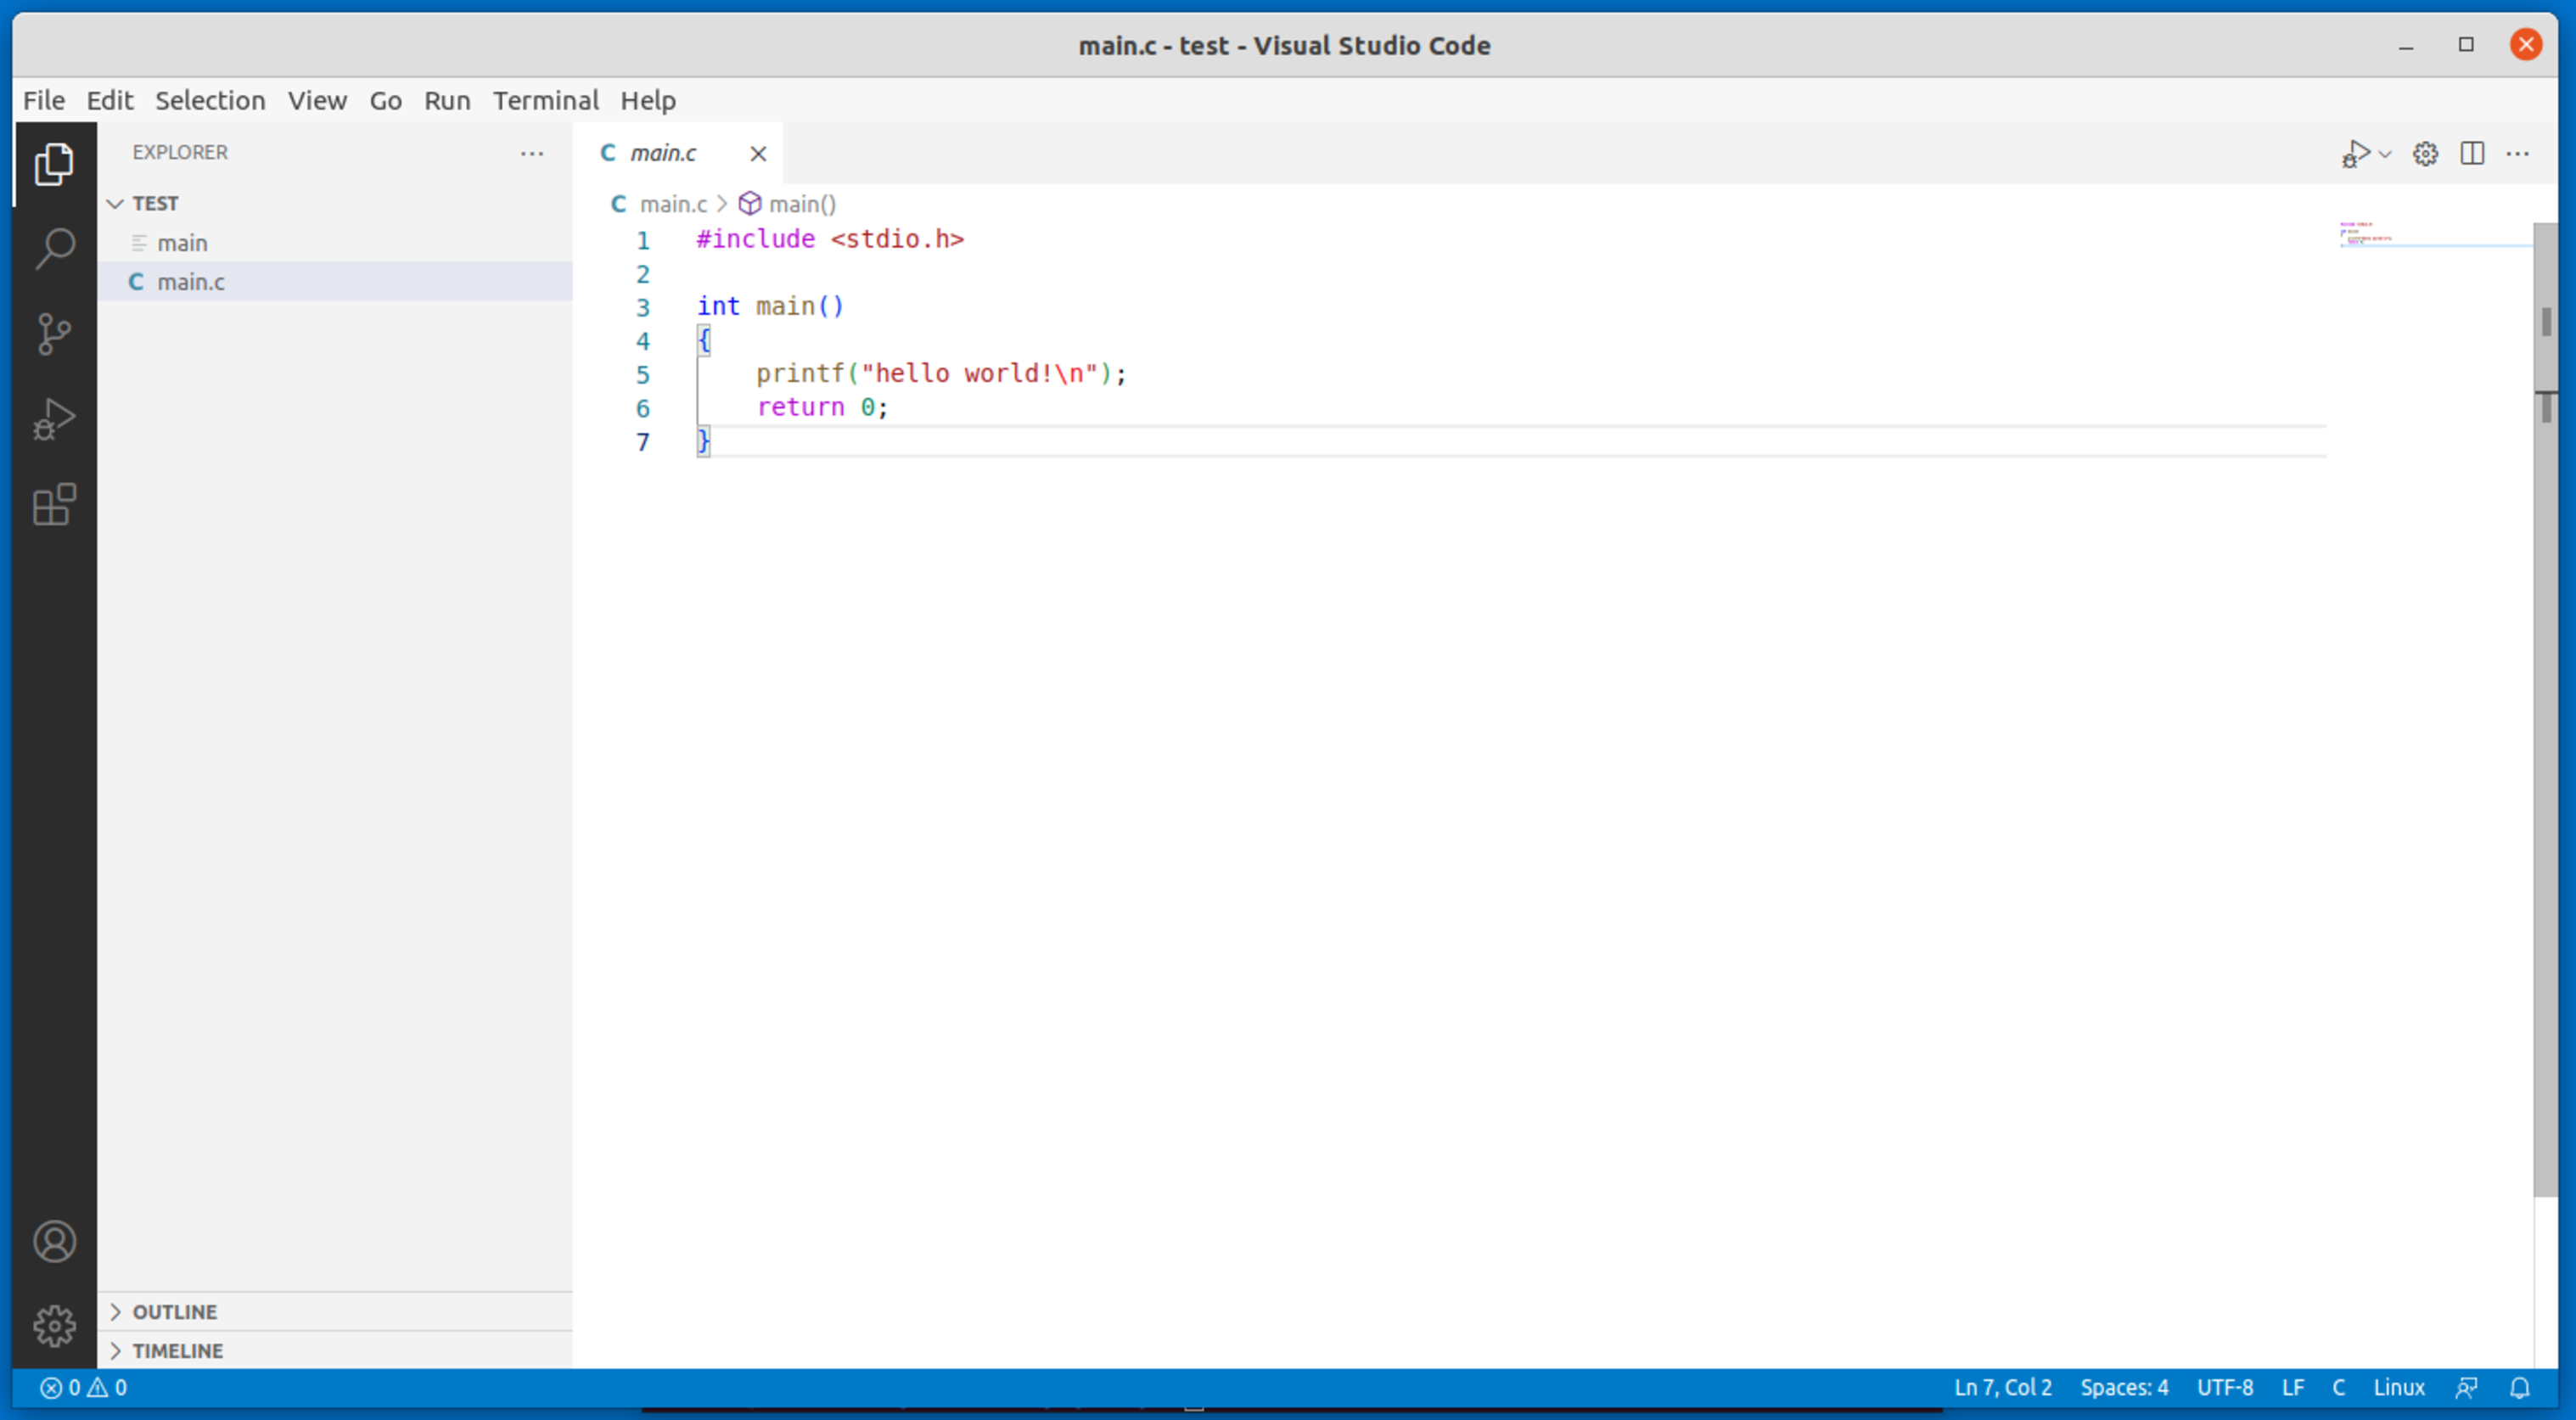
\includegraphics[width=0.8\linewidth]{figs/vscode.pdf}
			\end{figure}
		\end{center}
	\end{figure}
	\begin{itemize}
		\item {VS code is the most powerful and convenient Editor\footnote{https://code.visualstudio.com/download}}
		\item {One editor for designed for various programming languages, C, C++, Python and Java, etc}
	\end{itemize}
\end{frame}
